\section[Fundamental Concepts]{\hyperlink{toc}{Fundamental Concepts}}
\subsection{The beginnings of quantum mechanics}
Before we dive headfirst into the formalism of quantum mechanics, let us first review the first steps of the field as taken in the early 1900s. 

Our first founder is Max Planck; the problem at hand was the problem of the blackbody radiation spectrum. The two pre-existing laws (derived from thermodynamics arguments alone) predicting the BBR intensity as a function of frequency were flawed. The first was Wien's law (1896):
\begin{equation}
    I_{\text{Wien}}(f, T) \sim f^3\exp(-\frac{f}{T})
\end{equation}
which agreed with high frequency data well but failed to accurately describe low frequency emission. The second was Rayleigh-Jeans' law (1900):
\begin{equation}
    I_{\text{RJ}}(f, T) \sim f^4 T
\end{equation}
which agreed with low frequency data well but failed to accurately describe high frequency emission\footnote{It should be noted however that a full-derivation of the Rayleigh-Jeans law did not occur until 1905, at which point Planck had already established the more correct explanation.}. In fact, the intensity as predicted by Rayleigh-Jeans' diverges at high $\nu$, leading to the (obviously) erroneous conclusion that the total energy emitted by a black body is infinite; the so-called ``ultraviolet catastrophe''.

In order to solve this problem, in 1900 Planck proposed a quantum hypothesis; that light carries energy in individual packets, or quanta. In particular, for light of frequency $f$, each quanta carries energy:
\begin{equation}
    E = hf.
\end{equation}
Combining this quantum hypothesis with the Boltzmann supression of high-energy states (from thermodynamics), Planck's law was then derived to be:
\begin{equation}
    I_{\text{Planck}}(f, T) = \frac{2hf^3}{c^2}\frac{1}{\exp(\frac{hf}{k_B T}) - 1}
\end{equation}
which agrees with the BBR spectrum data across all frequencies\footnote{Further, we can observe that Planck's law agrees with Wien's law in the high-frequency limit, and with Rayleigh-Jeans' law in the low-frequency limit.}. It should also be noted that the integral over all $f$ of the above radiance law yields is finite, resolving the ultraviolet catastrophe. 

\begin{figure}[htbp]
    \centering
    TODO - plot of the three laws.
    \caption{<caption>}
    \label{fig-BBRspectra}
\end{figure}


\noindent
In the above discussion, we have introduced Planck's constant. It has numerical value\footnote{which is the set/absolute (rather than measured) value of the Planck constant as per the 2018 redefinition of SI units.}:
\begin{equation}
    h = 6.626070040 \times 10^{-34}\si{J.s}
\end{equation}
$h$ is quantified as ``small''. What exactly does small mean in this context? For comparison, $1\si{eV}$ is the kinetic energy of an electron acquired in a voltage drop of a Volt, $0.035\si{eV}$ is the average kinetic energy of an atom at room temperature (from $E_k = \frac{3}{2}k_B T$) and $2.4\si{eV}$ is the energy of a single photon from the middle of the visible spectrum ($600 \si{THz}$). The energy of a single photon, which depends on $h$, is in other words ``typical'' of microscopic phenomena.

Planck's quantum hypothesis would be confirmed in Einstein's (Nobel-prize winning) 1905 explanation of the photoelectric effect (which you likely covered in detail in a previous course in modern physics); namely that quanta of light transfer energy $E = hf$ to electrons in the metal, kicking them out\footnote{Provided of course that $hf > \Phi$ where $\Phi$ is the ``work function'' of the metal.}.

Our second founder of interest is DeBroglie. In 1924, he postulated that matter could behave like a wave, positing the DeBroglie wavelength relation:
\begin{equation}
    p = \frac{h}{\lambda}.
\end{equation}
The so-called ``wave-particle'' duality would be confirmed in 1927 by the Davisson-Germer experiment, which saw peaks of electron intensity at distinct angles, showing that electrons scatter in the same nature as photons.

Our third founder of interest is Schr\"{o}dinger, who postulated the Schr\"{o}dinger equation (expressed below in the position basis) in 1926:
\begin{equation}
    i\hbar \dpd{}{t}\Psi(\v{r}, t) = \left[\frac{-\hbar^2}{2m}\nabla^2 + V(\v{r}, t)\right] \Psi(\v{r}, t).
\end{equation}
It should be noted that this is one of the two core formulas of non-relativistic quantum mechanics, and is the quantum-mechanical equivalent of Newton's laws. It however does not cover the effects of special relativity (for which we defer the reader to a future course on quantum field theory) or quantum measurement (which we shall address now). 

An illuminating demonstration of quantum measurement takes the form of the Stern-Gerlach experiment (first carried out in 1921/1922; see \href{https://physicstoday.scitation.org/doi/10.1063/1.1650229}{this article} for more historical background). In this experiment, silver atoms are heated and escape from an oven with uniform velocity. The beam of atoms then pass through an inhomogenous magnetic field (generated by an asymmetric pair of magnetic pole pieces) where they are deflected, before hitting a screen where their position is recorded. 

\begin{figure}[htbp]
    \centering
    TODO - Sketch of the experiment
    \caption{Illustration of the Stern-Gerlach experiment.}
    \label{fig-SGexpsketch}
\end{figure}

Why are silver atoms used for this experiment? Moreover, what exactly is being measured? For this, we consider a simplified model of the atom (which will suffice for the purposes of explaining this experiment). Silver atoms consist of 47 electrons in the shell, and 47 protons and 61 neutrons in the nucleus. A first guess of the mechanism of the atoms being deflected by the magnetic field may be a Lorentz force effect; however this is not the case as the atoms are electrically neutral. Instead, the silver atom has a single unpaired electron which has an intrinsic angular momentum, known as spin. In particular, the electron is spin-1/2\footnote{We will return to a more detailed discussion of angular momentum and spin at a later portion of the course}. This provides the silver atom with a net magnetic moment $\gv{\mu}$ proportional to the electron spin\footnote{The astute reader may question why the spin of the unpaired proton in the nucleus has no contribution to the net magnetic moment. This is due to the fact that the proportionality factor between the spin and magnetic moment has a factor of inverse mass. Since the proton is 1836 times heavier than the electron, the proton's magnetic moment contribution is negligeble compared to the electron's.} $\v{S}$:

\begin{equation}
    \gv{\mu} \propto \v{S}.
\end{equation}
We then recall from electromagnetism that a magnetic dipole $\gv{\mu}$ in a magnetic field $\v{B}$ has interaction energy:
\begin{equation}
    E = -\gv{\mu} \cdot \v{B}.
\end{equation}
We can then find the force that the dipole feels by taking the (negative) gradient of the energy:
\begin{equation}
    \v{F} = -\gv{\nabla}(-\gv{\mu} \cdot \v{B}) = \mat{\dpd{}{x}(\gv{\mu} \cdot \v{B}) \\ \dpd{}{y}(\gv{\mu} \cdot \v{B}) \\ \dpd{}{z}(\gv{\mu} \cdot \v{B})}.
\end{equation}
Ignoring the magnetic fields that are not in the $z$-direction, we find the force on the silver atoms in the $z$-direction to be:
\begin{equation}
    F_z = \mu_z \dpd{B_z}{z}.
\end{equation}
So in the inhomogenous field produced by the asymmetric magnets, the silver atoms should feel an up/downwards force depending on the direction of $\v{S}$ (which determines $\mu_z$). 

\begin{figure}[htbp]
    \centering
    TODO - Picture
    \caption{The inhomogenous magnetic field used in the Stern-Gerlach experiment, which deflects the silver atoms due to their magnetic dipole moment proportional to electron spin.}
    \label{fig-SGexpmagnet}
\end{figure}

Classically, the magnetic moment $\v{\mu}$ can point in any direction, and therefore $\mu_z$ ranges continuously from $+\abs{\gv{\mu}}$ to $-\abs{\gv{\mu}}$. Hence, the signature we would expect on the Stern-Gerlach experiment screen (wherein the vertical position of the atoms on the screen corresponds to a measurement of the $z$-component of the magnetic moment) would be a continuous band, as seen in the left of Fig. 1.4 below. However, this is \emph{not} what is observed; instead the experimental result was two discrete dots with nothing in between, as seen in the right of the figure. 

\begin{figure}[htbp]
    \centering
    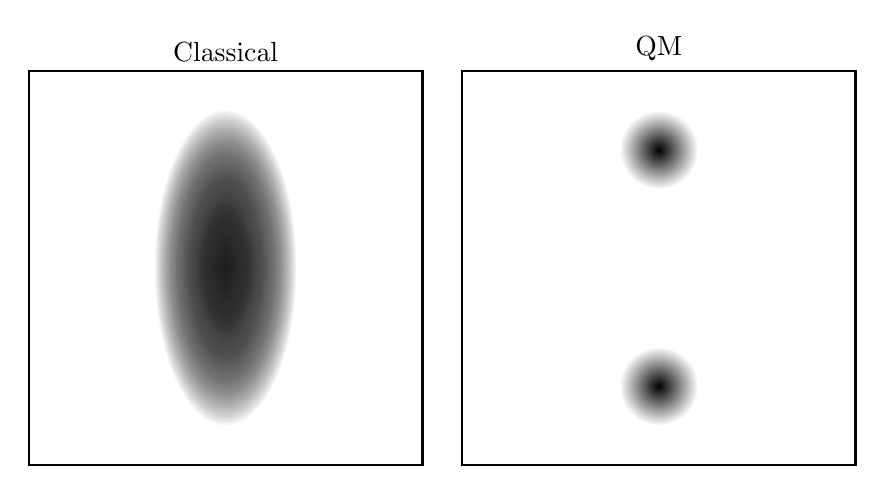
\begin{tikzpicture}[scale=1]
        \shade[even odd rule,inner color=black,outer color=white] (0,0) circle (0.5);
        \shade[even odd rule,inner color=black,outer color=white] (0,-3) circle (0.5);
        \draw[thick] (-2.5, -4) -- (-2.5, 1) -- (2.5, 1) -- (2.5, -4) -- cycle;
        \node[above] at (0, 1) {QM};

        \def\particles{(-5.5,-1.5) }
        \foreach \point in \particles{
        \foreach\i in {0,0.01,...,1.5} {
        \fill[opacity=\i*0.02,black] \point circle ({0.6-\i} and {1-2*\i});         
        }}
        \draw[thick] (-8, -4) -- (-8, 1) -- (-3, 1) -- (-3, -4) -- cycle;
        \node[above] at (-5.5, 1) {Classical};
    \end{tikzpicture}
    \caption{Classical prediction (left) and quantum mechanical prediction (right) for the Stern-Gerlach experiment. The screen on the right was observed in experiment.}
    \label{fig-SGexppredictions}
\end{figure}

How do we interpret this result? We can associate the top dot with spins fully polarized upwards ($\uparrow$) and the bottom dot with spins fully polarized downwards ($\downarrow$). But why is there no signature for sideways pointing spins? We first will answer how a general spin (1/2) state can be represented. If $\ket{\uparrow}$ represents the spin-up state and $\ket{\downarrow}$ represents the spin-down state, then a general spin (and hence sideways spins) can be represented as complex superpositions of these two states, i.e.
\begin{equation}
    \ket{\psi} = \alpha\ket{\uparrow} + \beta\ket{\downarrow}
\end{equation}
where $\alpha, \beta \in  \CC$. What happens in a measurement is then that one element of this general superposition is picked with some probability; indeed, quantum measurement is a probabilistic process. Specifically, we find according to the Born rule that the probability that we measure the spin to be up is $p(\uparrow) = \abs{\uparrow}^2$ and the probability that we measure the spin to be down is $p(\downarrow) = \abs{\downarrow}^2$. Since we require that we measure either spin-up or spin-down, we obtain the normalization condition:
\begin{equation}
    p(\uparrow) + p(\downarrow) = \abs{\alpha}^2 + \abs{\beta}^2 = 1.
\end{equation}
The spin state after the measurement is then $\ket{\uparrow}$ or $\ket{\downarrow}$ respectively, according to the Dirac projection postulate. We will return to these two postulates of quantum mechanics and discuss them in full generality shortly. 

However, we will however make a second comment about measurement before concluding this section. Namely, we consider the case where we perform a repeated measurement of the $z$-component of the spin. As discussed above, the initial general spin state is given by $\ket{\psi} = \alpha\ket{\uparrow} + \beta\ket{\downarrow}$. We then measure the $z$-component of spin and the post-measurement spin state is $\ket{\uparrow}$ or $\ket{\downarrow}$ with probability $\abs{\alpha}^2$ and $\abs{\beta}^2$ respectively. What happens if we measure the $z$-component of spin again? We might think that again, we have probability $\abs{\alpha}^2$ of measuring spin-up and probability $\abs{\beta}^2$ of measuring spin-down. But this is \emph{not} the case. If we measured spin-up in the first measurement, we will measure spin-up in the second measurement with probability one. Similarly, if we measured spin-down in the first measurement, we will measure spin-down in the second measurement with probability one. Evidently, the first measurement has done something to the spin such that the measurement probabilities for the second measurement have been affected (they are not the same as the first). This tells us that quantum measurement is a active process that influences the state of the system we measure. Specifically, it is an irreversible process; there is no notion of ``undo''-ing the measurement to recover the initial (pre-measurement) state.


\subsection{Kets, Bras, and Hilbert Space}
Our goal of the initial stages of this course will be to understand the following table:

\begin{table}[htbp]
    \centering\begin{tabular}{|c|c|}
        \hline Quantum states & $\ket{\psi} \in \H$ 
        \\ \hline Evolution & $i\hbar\pd{}{t}\ket{\psi} = H\ket{\psi}$
        \\ \hline Measurement & $\ket{\psi} \mapsto \frac{\Pi_j \ket{\psi}}{\sqrt{\bra{\psi}\Pi_j\ket{\psi}}} \quad p(j) = \bra{\psi}\Pi_j\ket{\psi}$
        \\ \hline
    \end{tabular}
    \caption{Axioms of quantum mechanics, concerning states, evolution, and measurement.}
    \label{table-QMaxioms}
\end{table}

We will discuss the axioms for quantum states and quantum measurement in this chapter, and the axiom for quantum evolution (which readers may recognize as the Schr\"{o}dinger equation in basis independent form) in the next. It is worth noting that these are the \emph{fundamental postulates} of quantum mechanics; like Newton's laws of motion in classical mechanics, they cannot be derived. We are only able to interpret them, check if they are consistent, and work out the implications.

Let's start the axiom for quantum states; after all it will helpful to know what the objects of our interest are, before we start to work with them! 

\begin{axiombox}{: Quantum states}\label{axiom-states}
    Quantum states $\ket{\psi}$ are vectors (also called ``kets'') in a complex Hilbert space $\H$.
\end{axiombox}

The above axiom is only meaningful if we know what a Hilbert space is; its definition is below:

\begin{defbox}{: (Complex) Hilbert spaces}\label{def-Hilbertspaces}
    $\H$ is a (complex) Hilbert space if:
    \begin{enumerate}[(i)]
        \item $\H$ is a vector space over $\CC$
        \item $\H$ has an inner product
        \item $\H$ is complete (with respect to the metric induced by the norm induced by the inner product)\footnotemark - For the purposes of this course, this last point can be ignored.
    \end{enumerate}
\end{defbox}
\footnotetext{This is a technical qualification for the mathematicians in the crowd. An intuitive explanation for the curious; the inner product on a Hilbert spaces creates a notion of distance on the space. There are sequences (of vectors) that get closer together over time; completeness tells us that any such sequences (known as Cauchy sequences) must converge to a limit.}

Note that the vector space axioms for closure imply that $\forall \ket{\psi}, \ket{\phi} \in \H$ (where $\forall$ means ``for all'') and $\forall c \in \CC$, then $\ket{\psi} + \ket{\phi} \in \H$ and $c\ket{\psi} \in \H$. This tells us that the superposition of quantum states is well defined!

An example which we will return to time and time again (and have already encountered once) is the Hilbert space for a spin-1/2 system. In this case, $\H = \CC^2$. A question that may be brooding in the reader's mind may be ``why do we have to use complex numbers?''; one may indeed wonder if real Hilbert spaces may suffice to do quantum mechanics. The response is negative; we indeed need complex numbers! As an illustrative example, consider again the general spin-1/2 state $\ket{\psi} = \alpha\ket{\uparrow} + \beta\ket{\downarrow}$. Suppose we want a state that has equal probability to be measured spin-up or spin-down under a measurement of the $z$-component of spin. Since $p(\uparrow) = \abs{\alpha}^2$ and $p(\downarrow) = \abs{\beta}^2$, in order to have equal probability we must have $\abs{\alpha} = 1/\sqrt{2}$ and $\abs{\beta} = 1/\sqrt{2}$. A spin pointing in the $+x$ or $-x$ directions indeed has equal weight of up and down. Up to an overall (irrelevant) minus sign, without using complex numbers there are two ways to superimpose $\ket{\uparrow}$ and $\ket{\downarrow}$, from which we can define states corresponding to spins fully polarized in $\pm x$:

\begin{equation}\label{eq-xpm}
    \ket{x, \pm} = \frac{\ket{\uparrow} \pm \ket{\downarrow}}{\sqrt{2}}.
\end{equation}
However, the $\pm \hat{x}$ and $\pm \hat{y}$ vectors lie in the same $z = 0$ plane, and by symmetry we should require that the $\ket{y, \pm}$ would also have equal weights of $\ket{\uparrow}$ and $\ket{\downarrow}$. But if we limit ourselves to real numbers only, we have already exhausted all possible equal-weight combinations of $\ket{\uparrow}$ and $\ket{\downarrow}$ in Eq. \eqref{eq-xpm}. We therefore require complex  numbers to represent all possible states (and indeed, we find that $\ket{y, \pm} = \frac{\ket{\uparrow} \pm i \ket{\downarrow}}{2}$).

Having motivated the ``complex'' in the complex vector space part of the definition of Hilbert spaces, let us now motivate the inner product. We want some way to compare quantum states to one another. Our geometric intuition tells us that the states $\ket{\uparrow}$ and $\ket{\nearrow}$ are ``close'' to each other, while $\ket{\uparrow}$ and $\ket{\downarrow}$ are very ``different''. In order to make this intuition rigorous, we define the inner product, and as a prerequisite we define the dual correspondence.

\begin{defbox}{: Dual correspondence}\label{def-dualcorrespondence}
    To each vector space $\H$, there exists a dual vector space $\H^*$. There is a one-to-one correspondence\footnotemark between the kets $\ket{\psi} \in \H$ and the bras\footnotemark $\bra{\psi} \in \H^*$. We call this the \emph{dual correspondence}, and write it as follows:
    \begin{equation}
        \ket{\psi} \DC \bra{\psi}.
    \end{equation}
    It has the following properties:
    \begin{enumerate}[(i)]
        \item $\ket{\psi} + \ket{\phi} \DC \bra{\psi} + \bra{\phi}$
        \item $c\ket{\psi} \DC c^*\bra{\psi}$
    \end{enumerate}
    where the $*$ denotes complex conjugation.
\end{defbox}
\footnotetext{Formally, this follows from the Riesz Representation Theorem. But for the purposes of this course, we take this one-to-one correspondence as a postulate. Curious readers can find discussions/proofs of the theorem in any text on functional analysis, or mathematical quantum theory.}
\footnotetext{Given such names because $\braket{}{}$ is a bracket - bra-ket. Physicists remain unmatched in their sense of humour.}

Having established the dual correspondence, we may now define the inner product:

\begin{defbox}{: Inner Product}\label{def-innerproduct}
    We define the inner product between $\ket{\psi} \in \H$ and $\ket{\phi} \in \H$ as:
    \begin{equation}
        \braket{\phi}{\psi} \in \CC
    \end{equation}
    with the properties:
    \begin{enumerate}[(i)]
        \item $\braket{\phi}{\psi} = \braket{\psi}{\phi}^*$
        \item $\braket{\psi}{\psi} \geq 0, \forall \ket{\psi} \in \H$
        \item $\braket{\psi}{\psi} = 0 \implies \ket{\psi} = \v{0}$.
    \end{enumerate}
\end{defbox}
Note that $\v{0}$ in the above definition is the null ket (also known as the zero vector, which must be an element of the Hilbert space), where $\v{0} = 0\ket{\psi}, \forall \ket{\psi}$. It is an unphysical state. We normally work with normalized states, i.e. states $\ket{\psi}$ that satisfy $\braket{\psi}{\psi} = 1$. The null ket has inner product zero and cannot be normalized.

As a first use of the inner product, let us return to our initial motivation for obtaining the ``likeness'' of states. For normalized states, it follows (and we will later prove) that:
\begin{equation}
    0 \leq \abs{\braket{\phi}{\psi}} \leq 1.
\end{equation}
We therefore can use the inner product as a method to evaluate the likeness of states. $\braket{\phi}{\psi} = 0$ means that $\ket{\psi}$ and $\ket{\phi}$ are maximally different, and $\abs{\braket{\phi}{\psi}} = 1$ corresponds to $\ket{\psi}$ and $\ket{\phi}$ being the same.